\documentclass[10pt,a4paper]{article}
\usepackage[utf8]{inputenc}
\usepackage[german]{babel}
\usepackage{mathrsfs}
\usepackage{amsmath}
\usepackage{amsfonts}
\usepackage{amssymb}
\usepackage{amsthm}
\usepackage[left=2cm,right=2cm,top=2cm,bottom=2cm]{geometry}
\usepackage{graphicx}

\begin{document}

\section{Aufgabe 11}

\section{Aufgabe 12}

\section{Aufgabe 13}

Die Stützstellen sind
\begin{equation}
  (-5, \frac{1}{26}), (-3, \frac{1}{10}), (-1, \frac{1}{2}), (1, \frac{1}{2}), (3, \frac{1}{10}), (5, \frac{1}{26})
\end{equation}
Dann ist das lineare Gleichungssystem
\begin{equation}
  \begin{pmatrix}
    2 & \frac{1}{2} & 0 & 0 & 0 & 0\\
    \frac{1}{2} & 2 & \frac{1}{2} & 0 & 0 & 0\\
    0 & \frac{1}{2} & 2 & \frac{1}{2} & 0 & 0\\
    0 & 0 & \frac{1}{2} & 2 & \frac{1}{2} & 0\\
    0 & 0 & 0 & \frac{1}{2} & 2 & \frac{1}{2}\\
    0 & 0 & 0 & 0 & \frac{1}{2} & 2
  \end{pmatrix}
  \cdot
  \begin{pmatrix}
    v_{1}\\
    v_{2}\\
    v_{3}\\
    v_{4}\\
    v_{5}\\
    v_{6}
  \end{pmatrix}
  =
  \frac{3}{4} \cdot
  \begin{pmatrix}
    \frac{1}{10}\\
    \frac{6}{13}\\
    \frac{2}{5}\\
    -\frac{2}{5}\\
    -\frac{6}{13}\\
    -\frac{1}{10}
  \end{pmatrix}
  =
  \begin{pmatrix}
    \frac{3}{40}\\
    \frac{9}{26}\\
    \frac{3}{10}\\
    -\frac{3}{10}\\
    -\frac{9}{26}\\
    -\frac{3}{40}
  \end{pmatrix}
\end{equation}

Die Lösung ist
\begin{equation}
  \begin{pmatrix}
    v_{1}\\
    v_{2}\\
    v_{3}\\
    v_{4}\\
    v_{5}\\
    v_{6}
  \end{pmatrix}
  =
  \begin{pmatrix}
    \frac{9}{2132}\\
    \frac{1419}{10660}\\
    \frac{1659}{10660}\\
    -\frac{1659}{10660}\\
    -\frac{1419}{10660}\\
    -\frac{9}{2132}
  \end{pmatrix}
\end{equation}

Die einzelnen Polynome sehen also wie folgt aus
\begin{align*}
  p_{1}(x) = & (1 - \frac{x + 5}{2}) \cdot \frac{1}{26} + \frac{x + 5}{2} \cdot \frac{1}{10}\\
  & + \frac{x + 5}{2} \cdot (1 - \frac{x + 5}{2}) \cdot ((2 \cdot \frac{9}{2132} - (\frac{1}{10} - \frac{1}{26})) (1 - \frac{x + 5}{2})\\
  & + ((-2\frac{1419}{10660} + (\frac{1}{10} - \frac{1}{26}))) \cdot \frac{x + 5}{2})
\end{align*}

Die restlichen schreibe ich mal nicht aus.

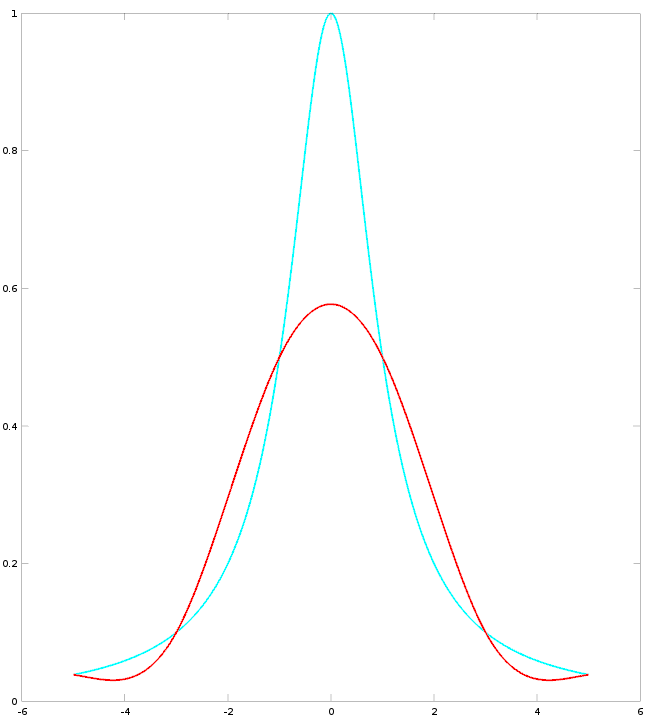
\includegraphics[width=300pt]{4_13.png}

\end{document}